\documentclass{article}

\usepackage{graphicx}
\usepackage{rotating}
\usepackage{amsmath}
\usepackage{fancyhdr}
\usepackage{listings}
\usepackage{xcolor}
\usepackage{color}
\usepackage{textcomp}
\usepackage{float}
\usepackage[sorting=none]{biblatex}
\usepackage[margin=1in]{geometry}
\usepackage[font={small,it}]{caption}
\usepackage{placeins}
\usepackage{xepersian}

%\DeclareMathOperator*{\btie}{\bowtie}
\addbibresource{bibliography.bib}
\settextfont[Scale=1.2]{B-NAZANIN.TTF}
\setlatintextfont[Scale=1]{Times New Roman}
\renewcommand{\baselinestretch}{1.5}
\pagestyle{fancy}
\fancyhf{}
\rhead{تکلیف هشتم درس شبکه‌های کامپیوتری 2}
\lhead{\thepage}
\rfoot{علیرضا ابره فروش}
\lfoot{9816603}
\renewcommand{\headrulewidth}{1pt}
\renewcommand{\footrulewidth}{1pt}
%%%%%%%%%%
\lstset
{
    language=[latex]tex,
    basicstyle=\ttfamily,
    commentstyle=\color{black},
    columns=fullflexible,
    keepspaces=true,
    upquote=true,
    showstringspaces=false,
    morestring=[s]\\\%,
    stringstyle=\color{black},
}
%%%%%%%%%%
%beginMatlab
\definecolor{mygreen}{RGB}{28,172,0} % color values Red, Green, Blue
\definecolor{mylilas}{RGB}{170,55,241}
%endMatlab
\begin{document}
%beginMatlab
\lstset{language=Matlab,%
    %basicstyle=\color{red},
    breaklines=true,%
    morekeywords={matlab2tikz},
    keywordstyle=\color{blue},%
    morekeywords=[2]{1}, keywordstyle=[2]{\color{black}},
    identifierstyle=\color{black},%
    stringstyle=\color{mylilas},
    commentstyle=\color{mygreen},%
    showstringspaces=false,%without this there will be a symbol in the places where there is a space
    numbers=left,%
    numberstyle={\tiny \color{black}},% size of the numbers
    numbersep=9pt, % this defines how far the numbers are from the text
    emph=[1]{for,end,break},emphstyle=[1]\color{red}, %some words to emphasise
    %emph=[2]{word1,word2}, emphstyle=[2]{style},    
}
%endMatlab
\begin{titlepage}
\begin{center}

\includegraphics[width=0.4\textwidth]{figures/IUT Logo.png}\\
        
\LARGE
\textbf{دانشگاه صنعتی اصفهان}\\
\textbf{دانشکده مهندسی برق و کامپیوتر}\\
        
\vfill
        
\huge
\textbf{عنوان: تکلیف چهارم درس ریزپردازنده}\\
        
\vfill
        
\LARGE
\textbf{نام و نام خانوادگی: علیرضا ابره فروش}\\
\textbf{شماره دانشجویی: 9816603}\\
\textbf{نیم\,سال تحصیلی: پاییز 1400}\\
\textbf{مدرّس: دکتر عارف کریمی افشار}\\
\end{center}
\end{titlepage}


%\tableofcontents
\newpage

\section{فصل 9}
\subsection{سوال 1}
\subsubsection{\lr{a}}
\begin{figure}[H]
    \centering
    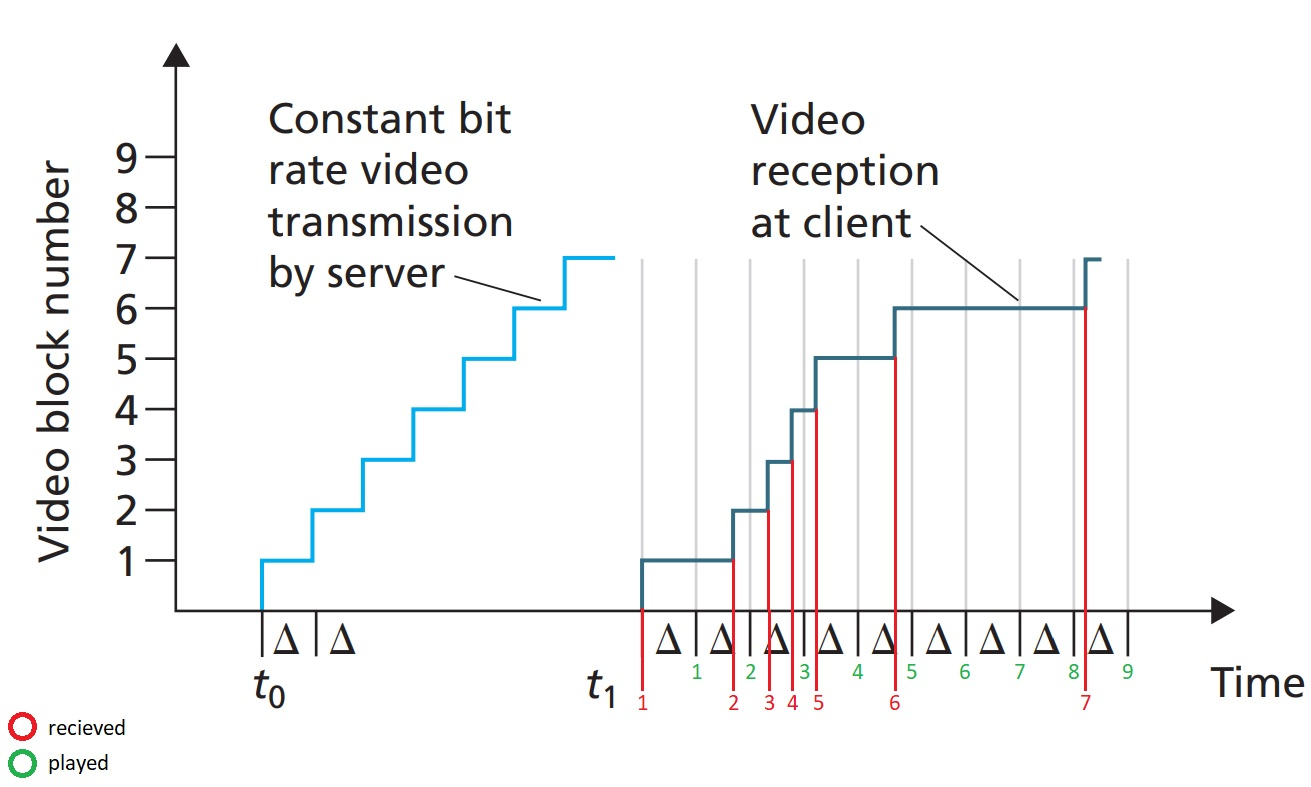
\includegraphics[width=1.0\textwidth]{figures/1a.jpg}
    \caption
	{}
    \label{fig:fig1}
\end{figure}
برای اینکه یک بلاک ویدئو بتواند در زمان مقرر اجرا شود باید قبل از اجرا به طور کامل دریافت شده باشد. در واقع اختلاف فاصله‌ی زمانی بین دریافت تا اجرای آن حداقل به اندازه‌ی $\Delta$ باشد. همانطور که در تصویر مشاهده می‌کنید این شرط تنها برای بلاک‌های با شماره‌ی 1، 4، 5 و 6 صدق می‌کند. پس تنها این بلاک‌ها در زمان مقرر خود اجرا می‌شوند.
\subsubsection{\lr{b}}
\begin{figure}[H]
    \centering
    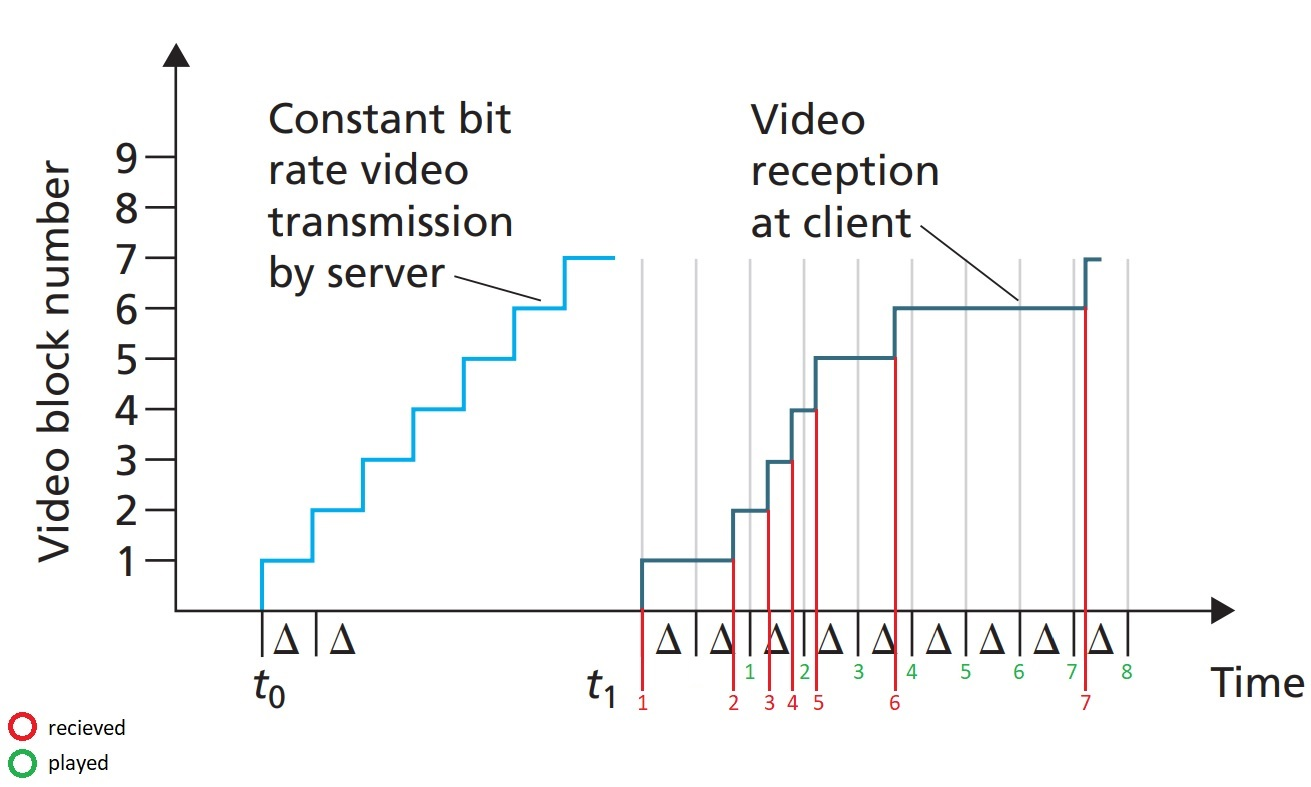
\includegraphics[width=1.0\textwidth]{figures/1b.jpg}
    \caption
	{}
    \label{fig:fig1}
\end{figure}
همانند قسمت قبل چون بلاک‌های 1 تا 6 قبل از شروع به اجرا دریافت شده‌اند پس تنها این بلاک‌ها در زمان مقرر خود اجرا می‌شوند.
\subsubsection{\lr{c}}
در سناریوی بالا بیشینه تعداد بلاک‌های ذخیره شده در بافر کلاینت برابر با 2 است. قبل از اجرای بلاک 3 در زمان $t_{1} + 3\Delta$ بلاک‌های 3 و 4، یا قبل از اجرای بلاک 4 در زمان $t_{1} + 4\Delta$ بلاک‌های 4 و 5 در کلاینت بافر شده‌اند.
\subsubsection{\lr{d}}
\begin{figure}[H]
    \centering
    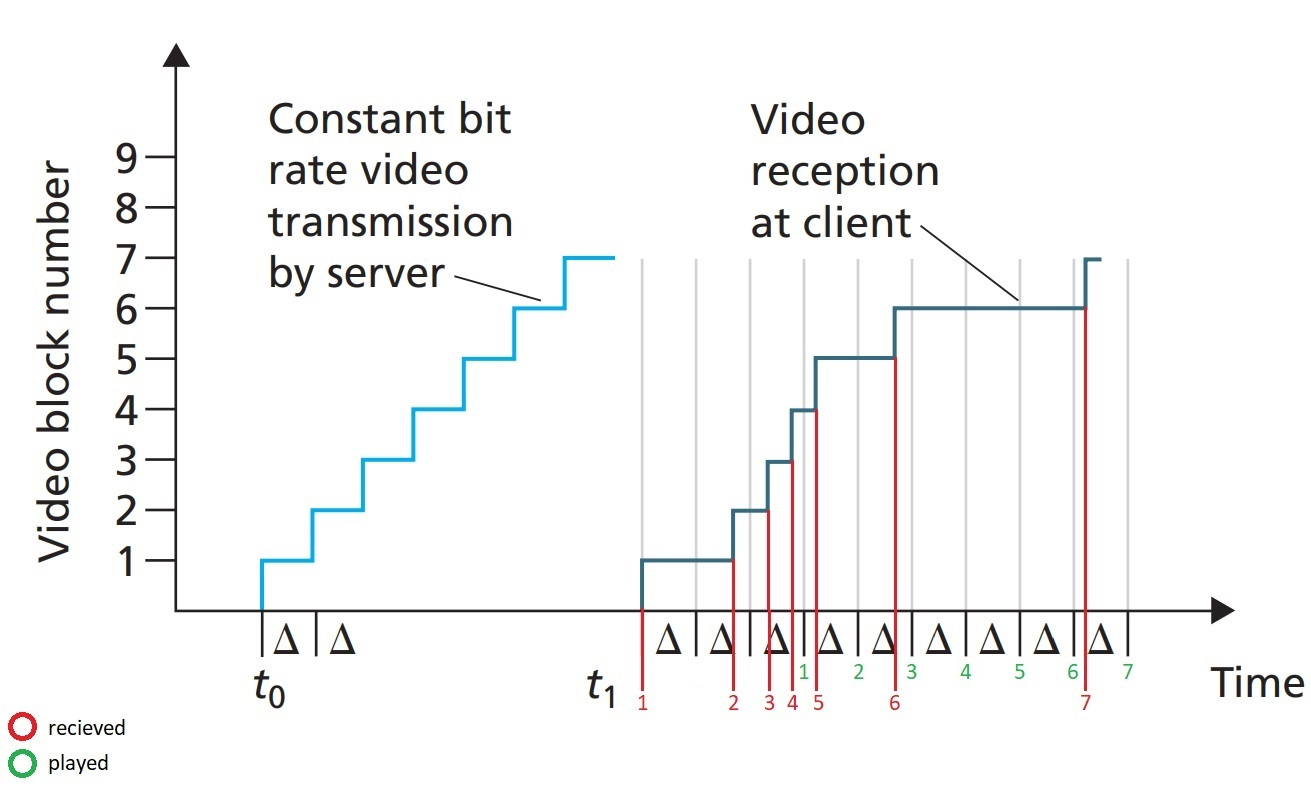
\includegraphics[width=1.0\textwidth]{figures/1d.jpg}
    \caption
	{}
    \label{fig:fig1}
\end{figure}
زمان‌بندی اجرای اولین بلاک باید به گونه‌ای باشد که بلاک با بیشترین تاخیر (بلاک 7) قبل از اجرا دریافت شده باشد. پس با توجه به شکل بالا بلاک اول باید در زمان $t_{1} + 3\Delta$ اجرا شود.

\subsection{سوال 6}
\subsubsection{\lr{a}}
در هر 20 میلی‌ثانیه $h + 160$ بایت فرستاده می‌شود. در نتیجه \lr{transmission rate} برابر است با:
$
\frac{(h+160)\times 8}{20}Kbps
$

\subsubsection{\lr{b}}
$
RTP = 12 B \\
IP = 20 B \\
UDP = 8 B
$

\subsection{سوال 10}
هر دو فرایند به هم شبیه هستند. هر دو فرمول یکسانی دارند و در نتیجه هر دو به ازای نمونه‌های گذشته وزن کاهنده دارند. یکی از تفاوت‌ها این است که در تخمین میانگین \lr{RTT}، زمانی که داده فرستاده می‌شود تا زمانی که \lr{Ack}ِ آن برمی‌گردد در یک ماشین ثبت می‌شود. برای تخمین تاخیر، دو مقدار گزارش‌شده روی دو ماشین متفاوت ثبت می‌شود. از این رو تاخیر نمونه می‌تواند منفی باشد.


\subsection{سوال 11}
\subsubsection{\lr{a}}
تاخیر پکت‌های 2 تا 8 به ترتیب، 7، 9، 8، 7، 9، 8 و بیشتر از 8 واحد زمانی است.

\subsubsection{\lr{b}}
\begin{figure}[H]
    \centering
    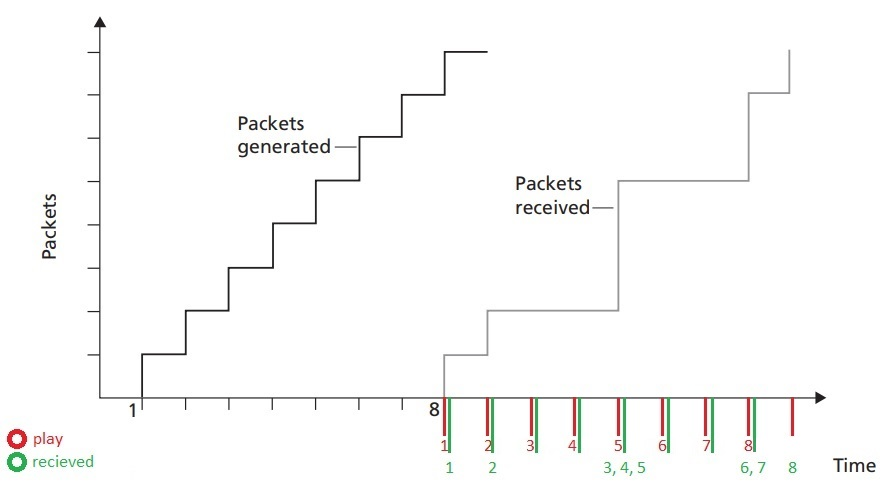
\includegraphics[width=1.0\textwidth]{figures/11b.jpg}
    \caption
	{}
    \label{fig:fig1}
\end{figure}
با توجه به تصویر بالا، پکت‌های 3، 4، 6، 7، و 8 قبل از زمان مقرر برای پخش نرسیده‌اند.

\subsubsection{\lr{c}}
\begin{figure}[H]
    \centering
    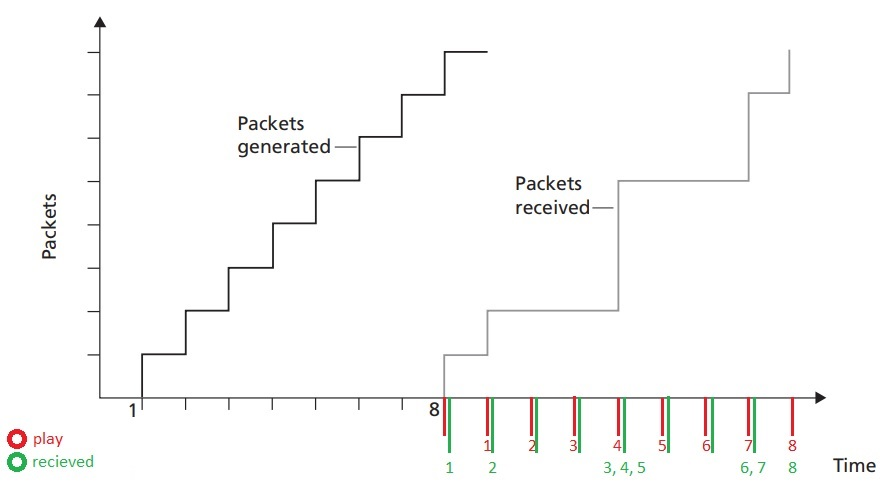
\includegraphics[width=1.0\textwidth]{figures/11c.jpg}
    \caption
	{}
    \label{fig:fig1}
\end{figure}
با توجه به تصویر بالا، پکت‌های 3 و 6 قبل از زمان مقرر برای پخش نرسیده‌اند.

\subsubsection{\lr{d}}
با توجه به قسمت قبل، اگر پخش با 2 واحد زمانی تاخیر (در $t=10$) صورت بگیرد همه‌ی 8 پکت اول قبل از زمان مقرر پخش دریافت شده‌اند.
%%%%%%%%%%%%%%%%%%%%%%%%%%%%%%%%%%%
%%%%%%%%%%%%%%%%%%%%%%%%%%%%%%%%%%%
%%%%%%%%%%%%%%%%%%%%%%%%%%%%%%%%%%%

\section*{منابع}
\renewcommand{\section}[2]{}%
\begin{thebibliography}{99} % assumes less than 100 references
%چنانچه مرجع فارسی نیز داشته باشید باید دستور فوق را فعال کنید و مراجع فارسی خود را بعد از این دستور وارد کنید


\begin{LTRitems}

\resetlatinfont

\bibitem{b1}
\end{LTRitems}

\end{thebibliography}


\end{document}
